\documentclass[9pt,twoside,lineno]{new_article}
% Use the lineno option to display guide line numbers if required.

\templatetype{supportinginfo}

\title{Genomic architecture controls multivariate adaptation to climate change}
\author{Drew E. Terasaki Hart and Ian J. Wang}
\correspondingauthor{Corresponding Author name.\\E-mail: drew.hart@berkeley.edu}

\begin{document}

\maketitle

%% Adds the main heading for the SI text. Comment out this line if you do not have any supporting information text.
%\SItext


%%% Each figure should be on its own page

\begin{figure*}
\centering
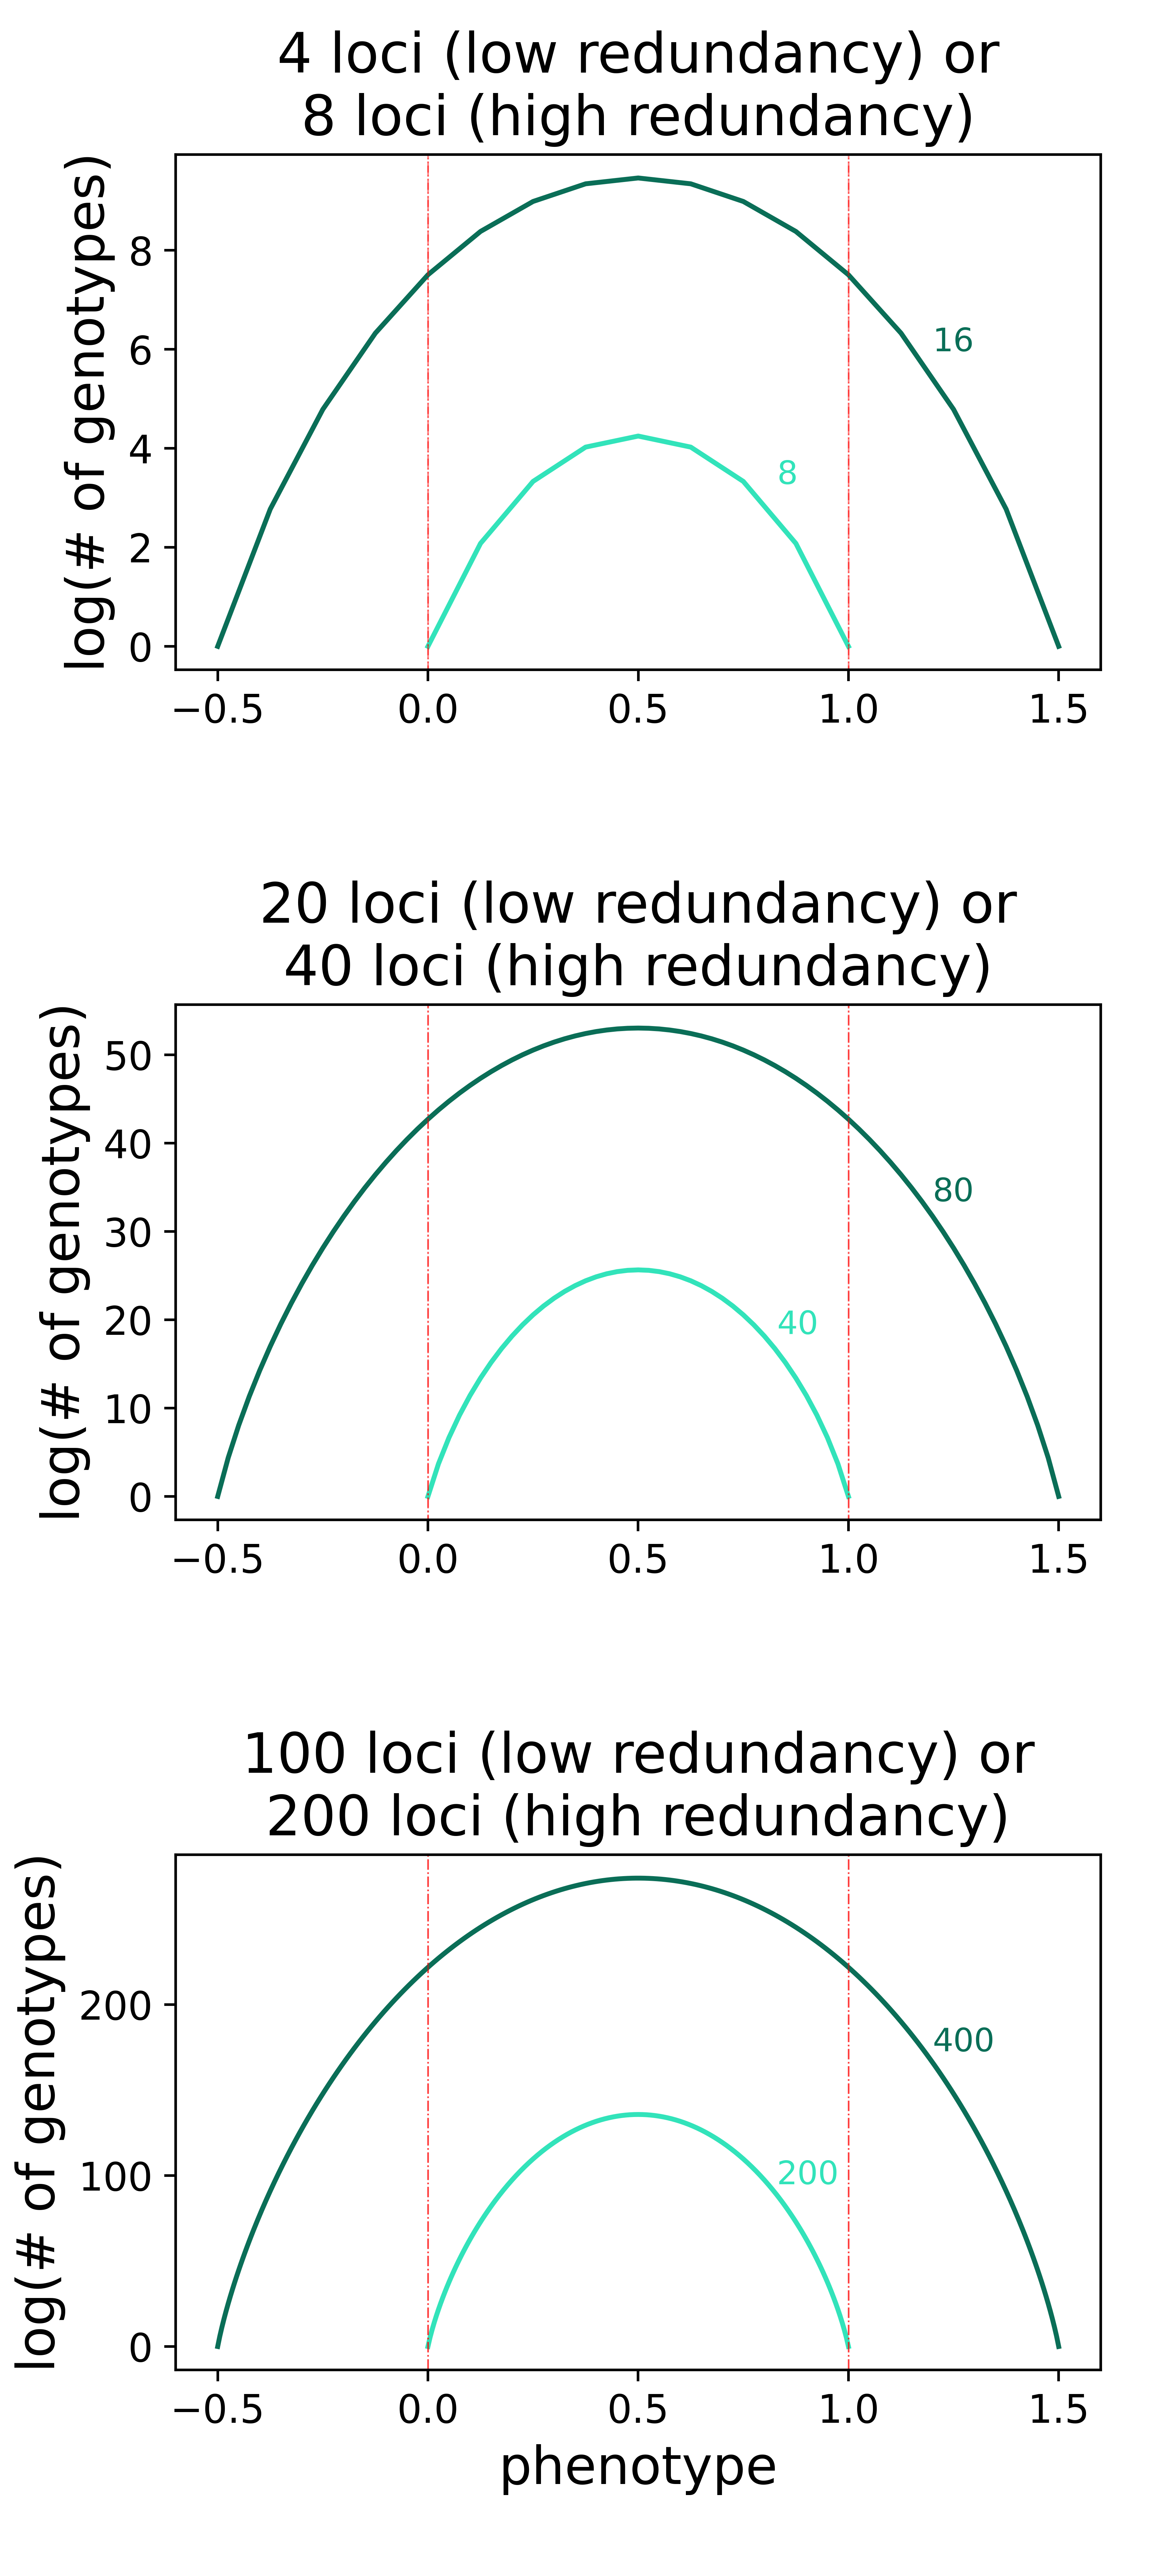
\includegraphics[width=.5\linewidth]{pub/figs_and_stats/FIG_S1_redundancy.png}
\caption{Plots of the number of genotypes (y-axis) that yield each phenotypic value (x-axis). Polygenicities corresponding to low redundancy scenarios are plotted and labeled in light teal and those corresponding to high redundancy scenarios in dark teal. The minimum and maximum environmental values on the landscape are represented by dashed vertical lines. Plots follow the visualization of genotypic redundancy in Láruson \textit{et al.} 2020 \cite{laruson}, Box 1, Figure I.
}
\label{fig:fig_s1}
\end{figure*}




\begin{figure*}
\centering
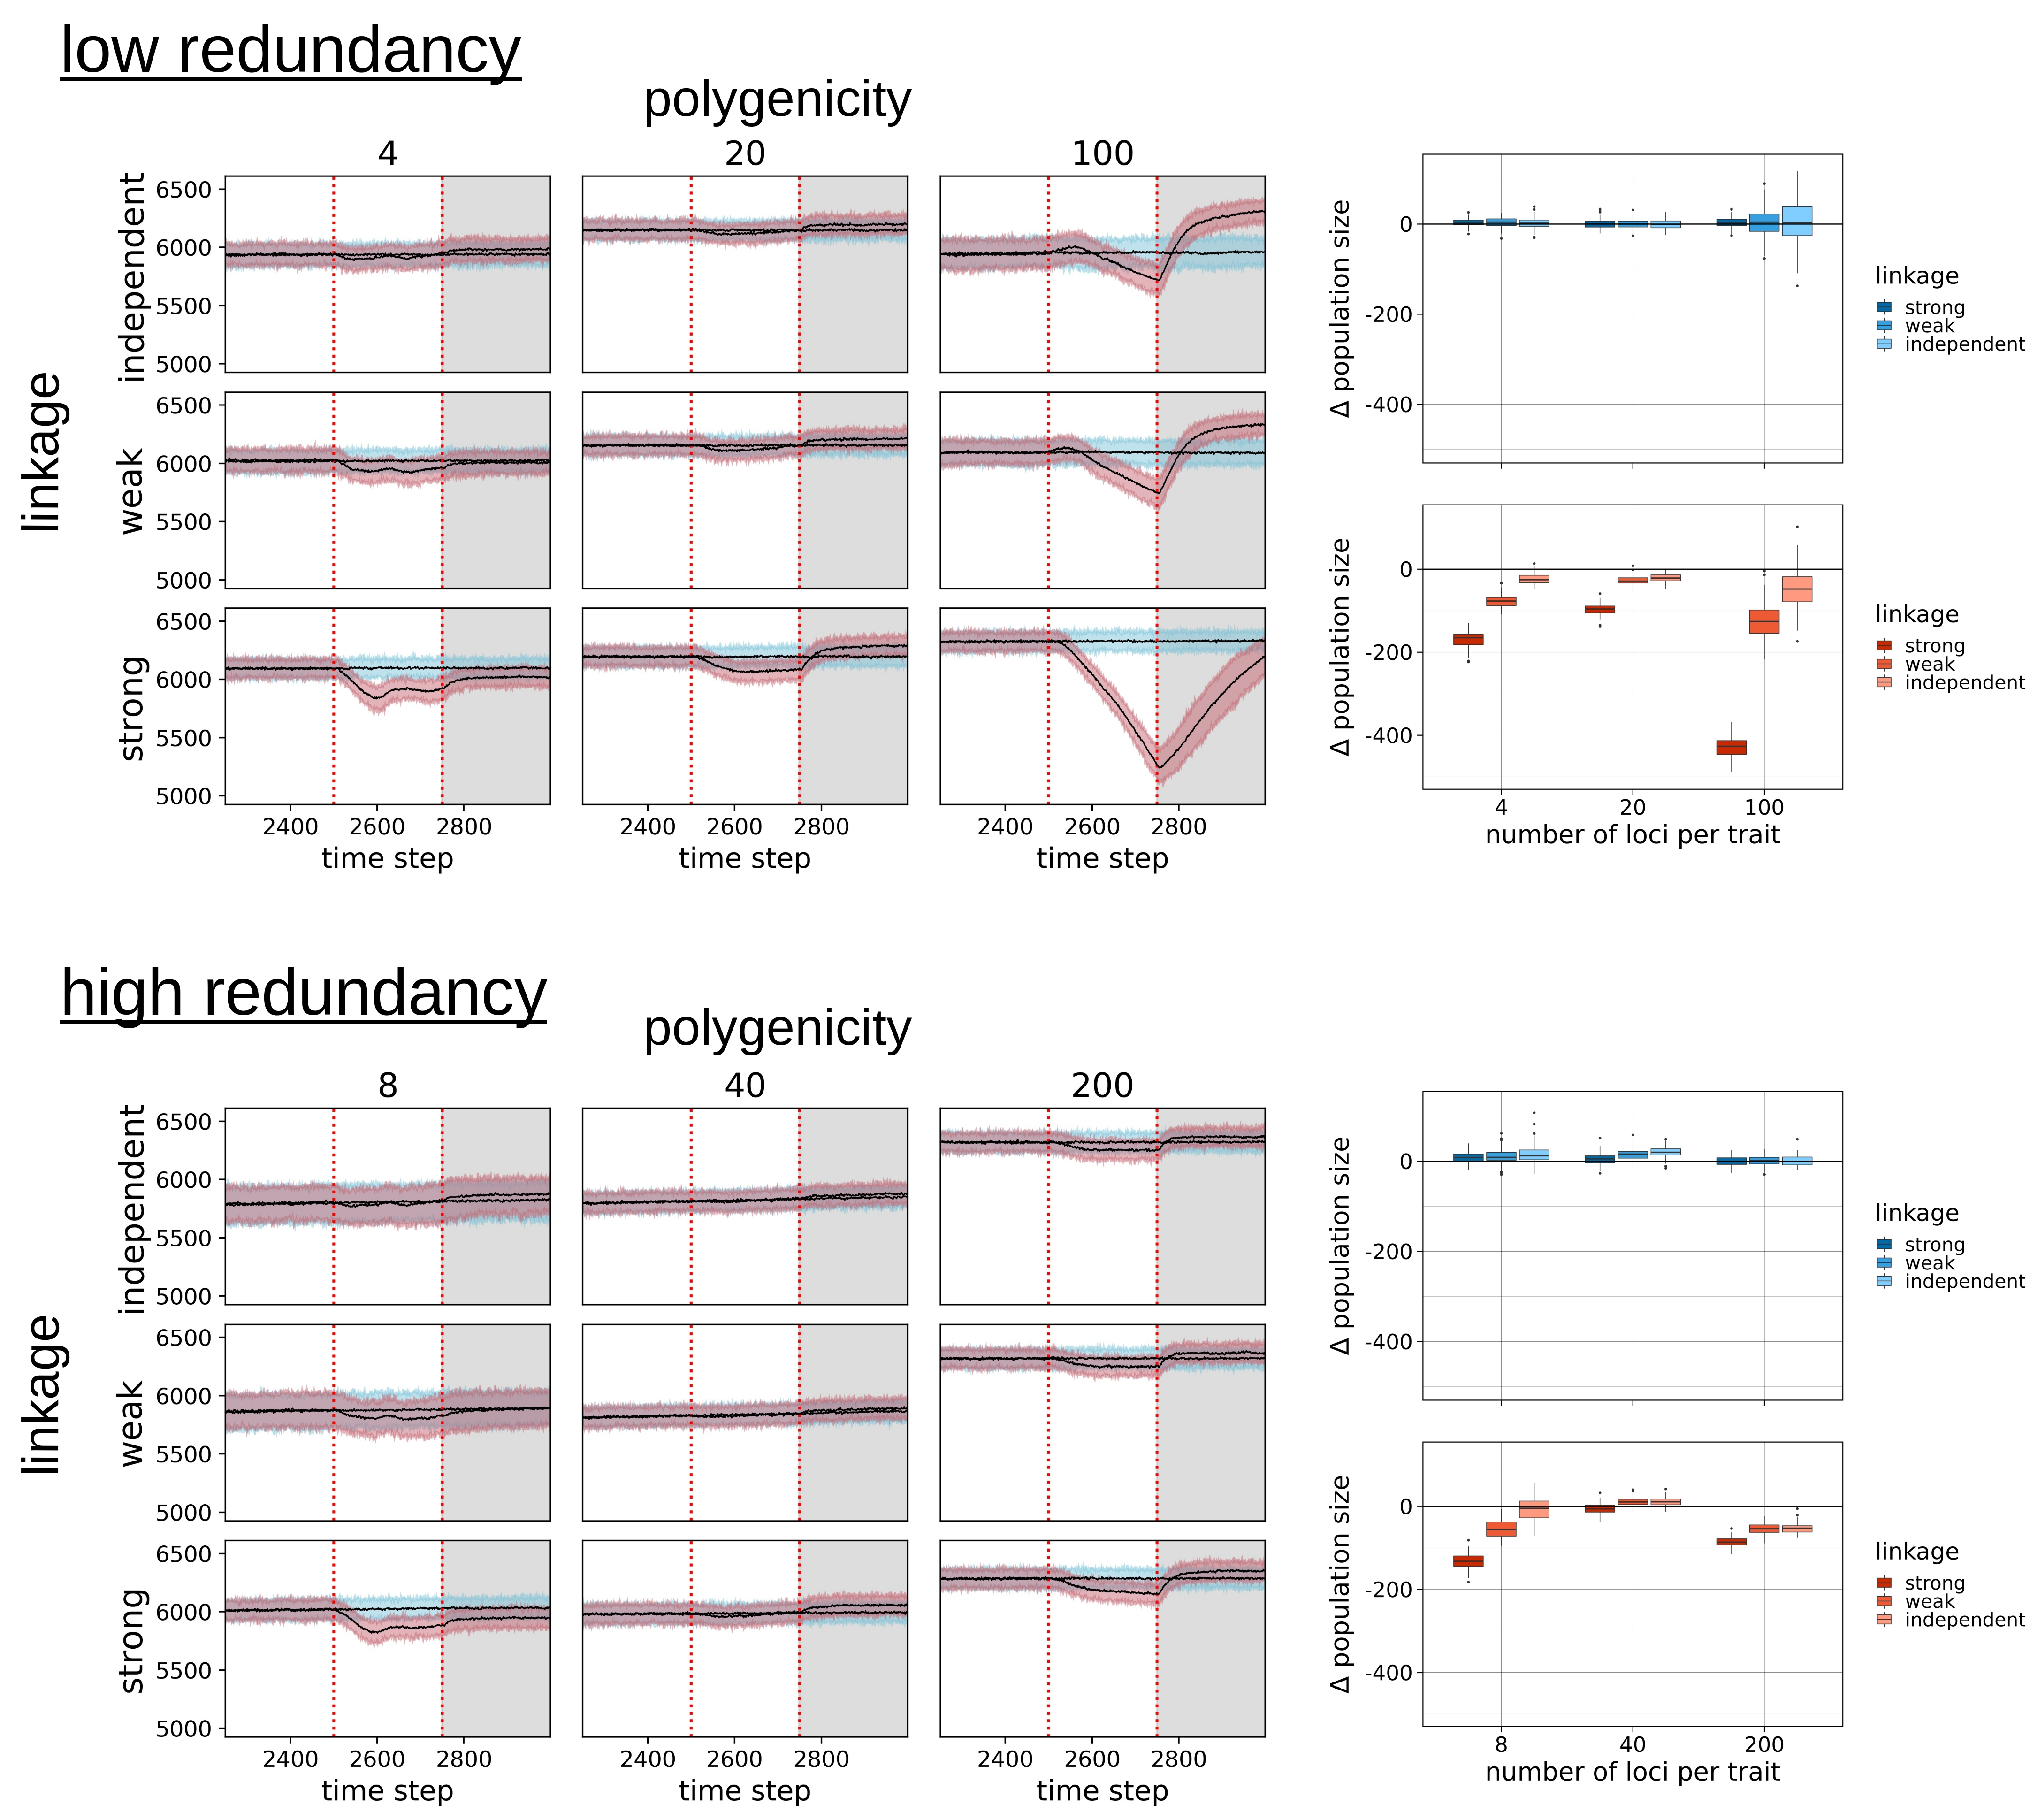
\includegraphics[width=15.8cm]{pub/figs_and_stats/FIG_S2_Nt_over_time.png}
\caption{Left: Population size dynamics for all scenarios during the 250 time steps before, during, and after the climate change period (separated by red, dashed lines). Black lines represent mean values, and the shaded areas represent variability envelopes (5th percentile to 95th percentile) for climate change (red) and null simulations (blue). Right: Boxplots of changes in mean population size
during the climate change period for all scenarios. Null scenarios are plotted on the top, in blue, and main scenarios are plotted on the bottom, in red. Within each plot, the
scenarios are organized by polygenicity (number of loci per trait) on the x-axis and shaded by the strength of linkage.}
\label{fig:fig_s2}
\end{figure*}



\begin{figure*}
\centering
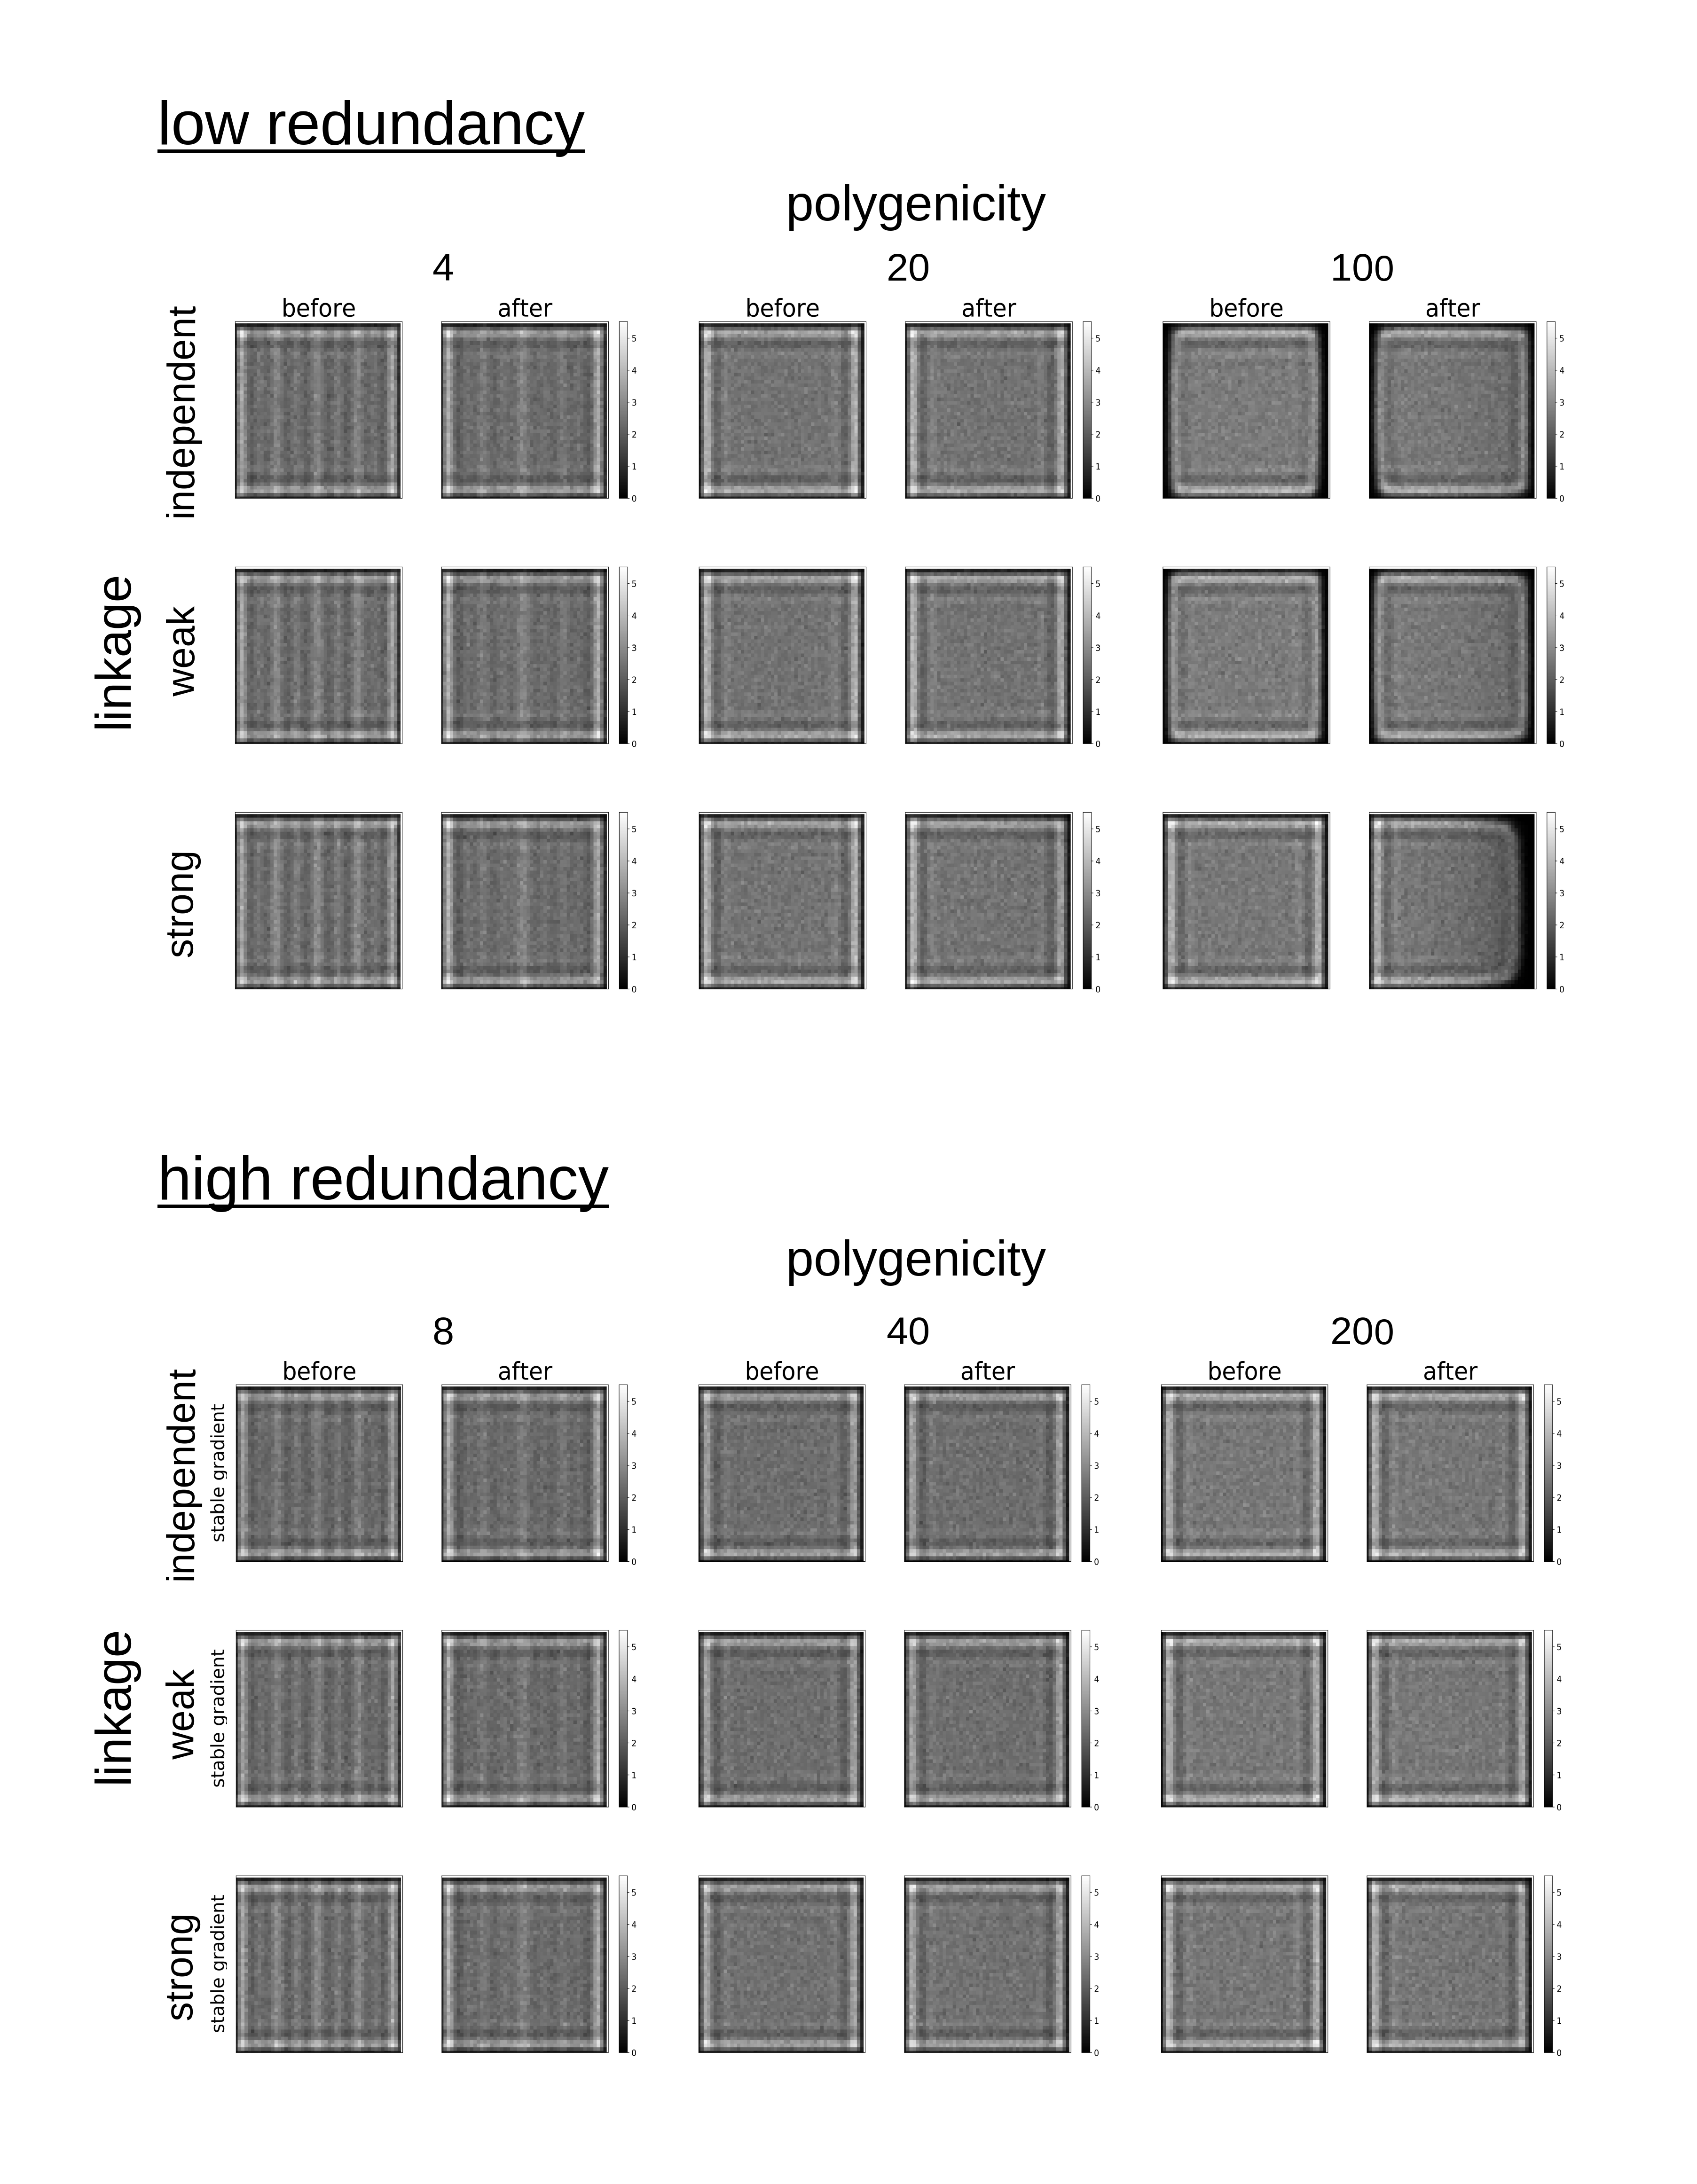
\includegraphics[width=.8\linewidth]{pub/figs_and_stats/FIG_S3_density_shift_ROWLABELS_CORRECTED.png}
\caption{Maps of population density before and after climate change for all scenarios. In addition to showing local extinction in the low redundancy, high polygenicity, strong linkage scenario (top section, bottom right), these maps also show moderate simulation edge effects and density banding in the low polygenicity scenarios because of the mismatch between environmental and phenotypic resolutions.}
\label{fig:fig_s3}
\end{figure*}



\begin{figure*}
\centering
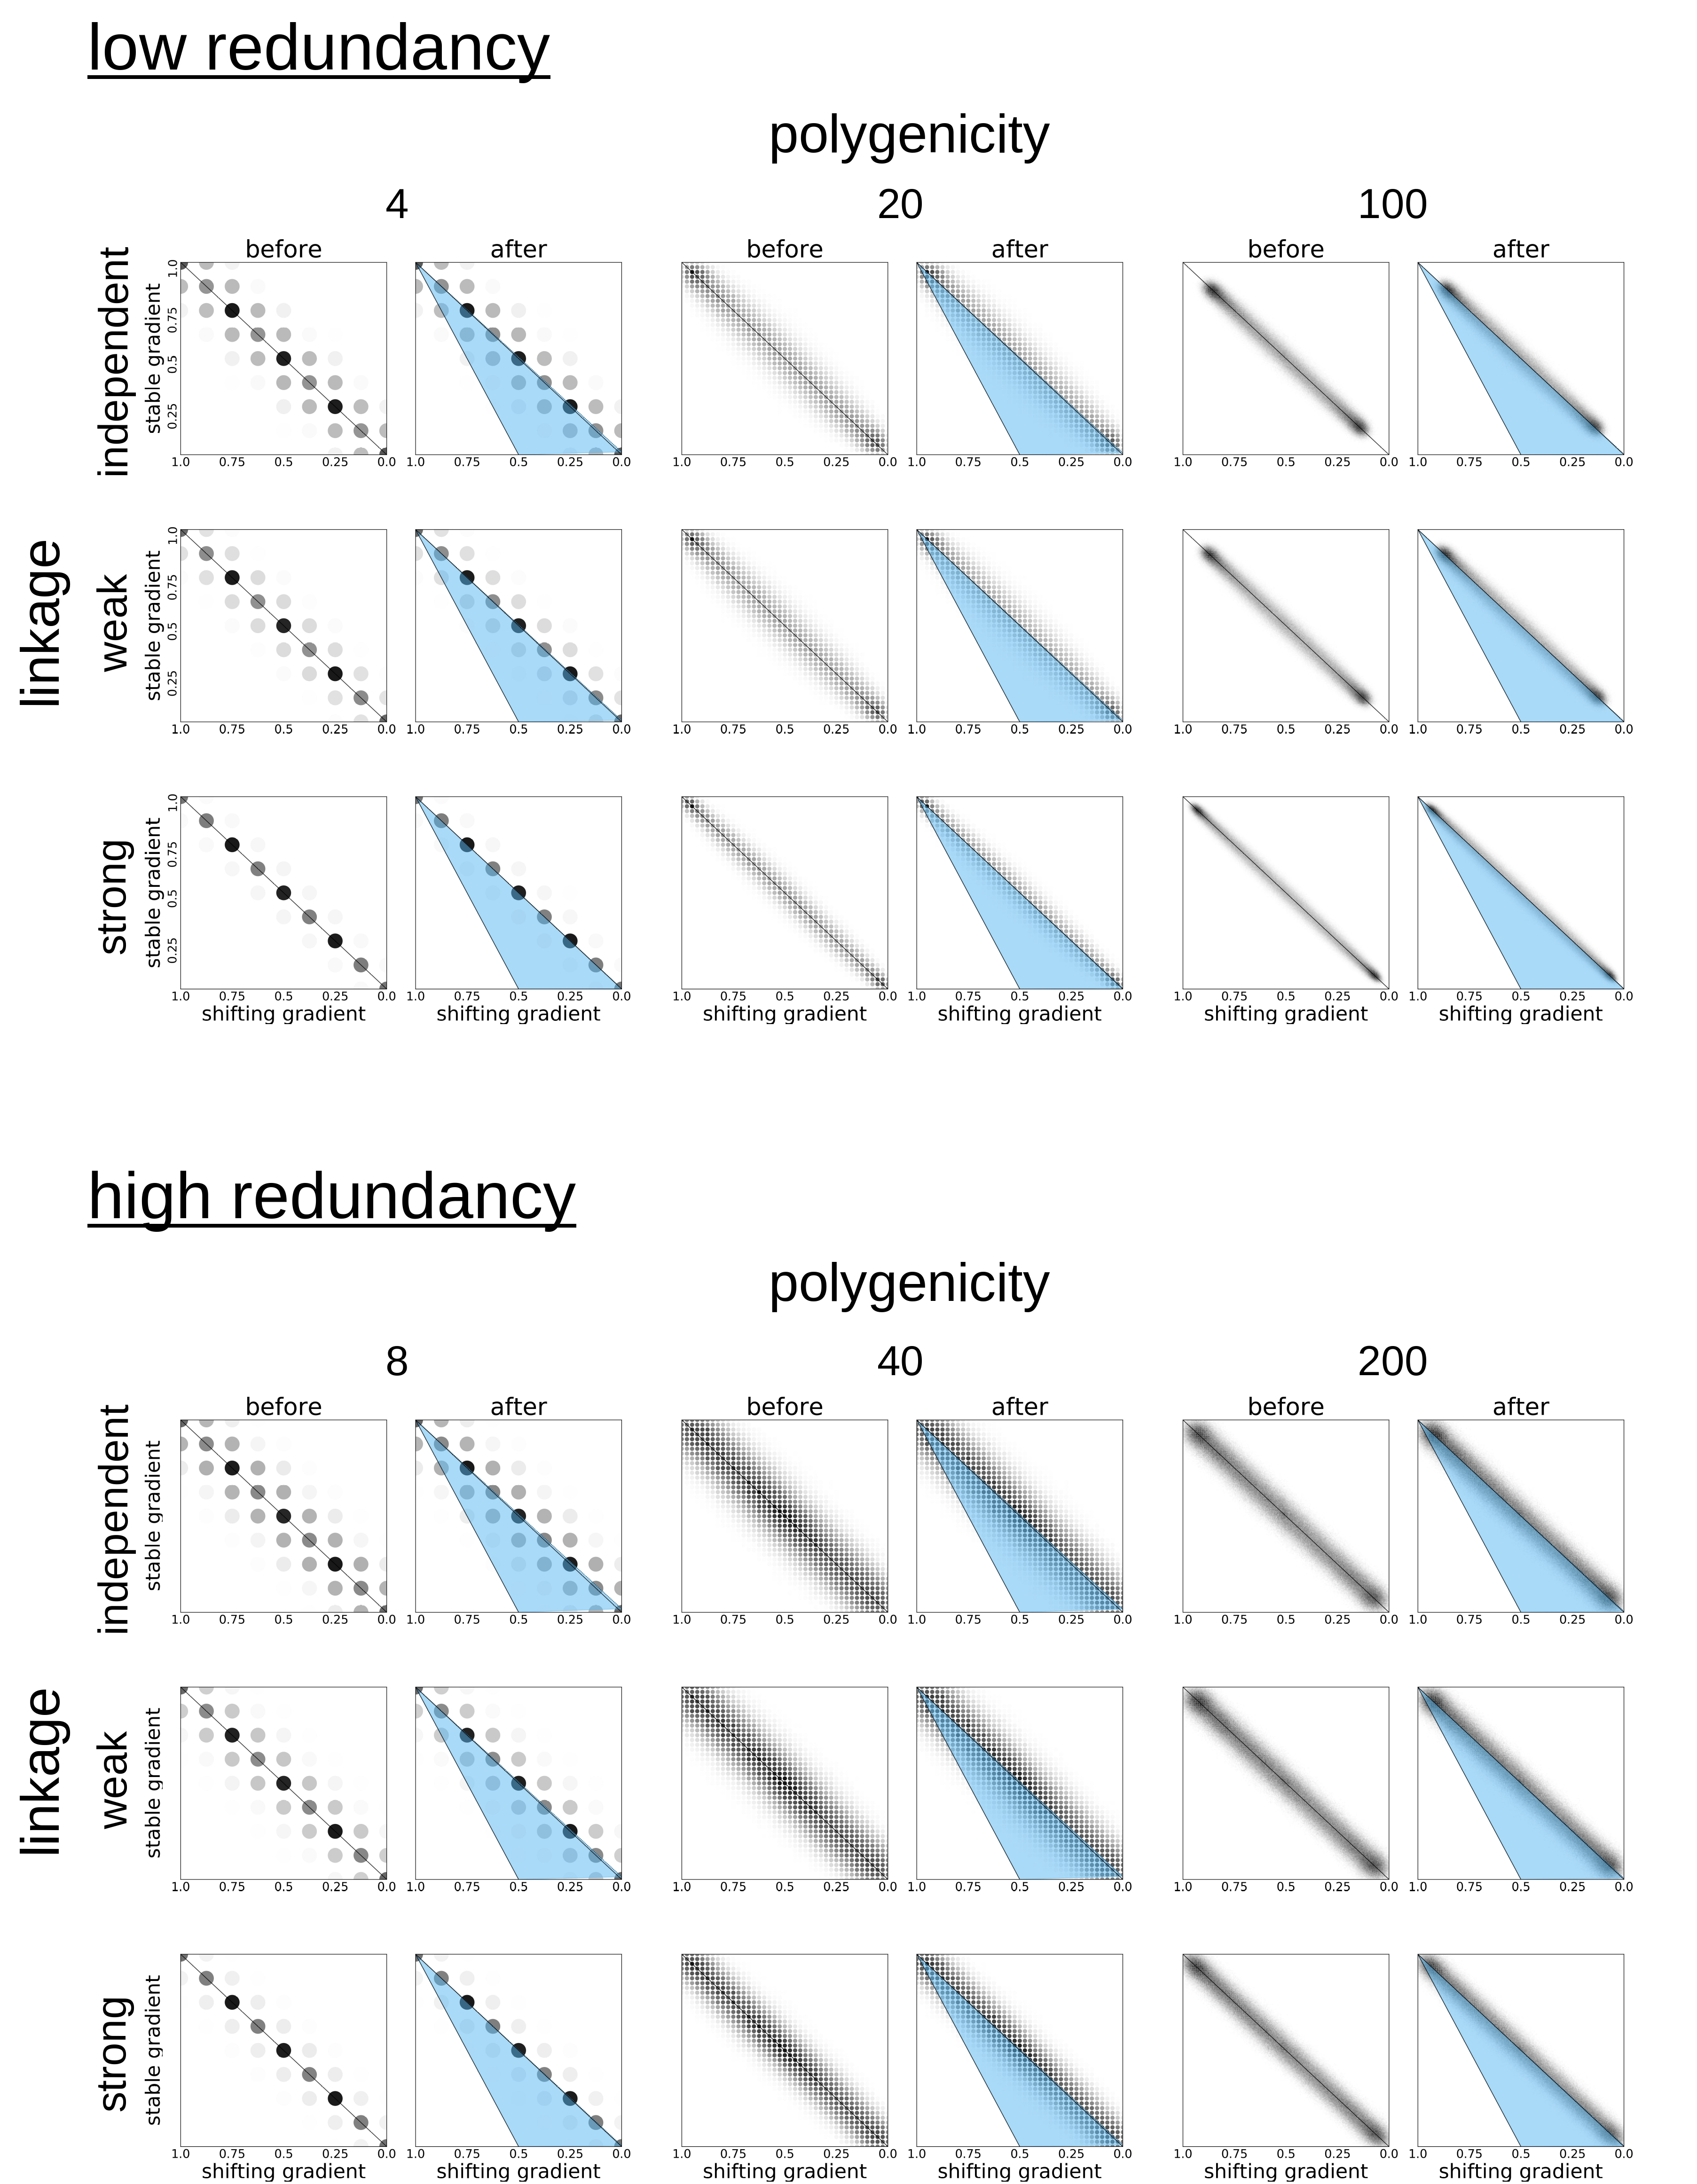
\includegraphics[width=.8\linewidth]{pub/figs_and_stats/FIG_S4_phenotypic_shift_null_ROWLABELS_CORRECTED.png}
    \caption{Scatterplots of the observed versus expected phenotypic shift during the climate change period for all 18 of our simulated scenarios. For each scenario, the left (’before’) scatterplot shows the distribution of phenotypes before climate change begins, and the right (’after’) scatterplot shows how the distribution has shifted by the end of the climate change period. The trait adapted to the shifting environmental gradient is distributed along the x-axis, with the trait adapted to the stable gradient on the y-axis. The size and opacity of each point represents the number of individuals exhibiting that two-dimensional phenotype. The gridded arrangement of the points in each scatterplot is a function of the number of loci per trait, which determines the set of possible phenotypes. Solid black lines delineate the shifts in the phenotypic distributions’ central tendencies that are expected to take place during the climate change period, dotted black lines depict the observed distributions’ central tendencies, and blue wedges depict the differences between the expected and observed distributions (‘phenotypic shortfall’).}
\label{fig:fig_s4}
\end{figure*}




\begin{table}\centering
\caption{\label{tab:tab_s1}Predicted main vs. null upslope gene flow (and 95\% confidence intervals) for all 18 scenarios.}
\begin{tabular}{|b{0.1\linewidth}|b{0.1\linewidth}|b{0.1\linewidth}|b{0.22\linewidth}|}
\hline
\textbf{genicity} & \textbf{linkage} & \textbf{redundancy} & \textbf{predicted gene flow ($\pm$ 95\% C.I.)} \\
\hline
0 & 2 & 1 & $0.04916 \pm 0.00211$ \\
1 & 2 & 1 & $0.03496 \pm 0.00177$ \\
2 & 2 & 1 & $0.02076 \pm 0.00211$ \\
0 & 1 & 1 & $0.03622 \pm 0.00177$ \\
1 & 1 & 1 & $0.02202 \pm 0.00134$ \\
2 & 1 & 1 & $0.00782 \pm 0.00177$ \\
0 & 0 & 1 & $0.02328 \pm 0.00211$ \\
1 & 0 & 1 & $0.00908 \pm 0.00177$ \\
2 & 0 & 1 & $-0.00512 \pm 0.00211$ \\
0 & 2 & 0 & $0.06470 \pm 0.00211$ \\
1 & 2 & 0 & $0.05050 \pm 0.00177$ \\
2 & 2 & 0 & $0.03630 \pm 0.00211$ \\
0 & 1 & 0 & $0.05176 \pm 0.00177$ \\
1 & 1 & 0 & $0.03756 \pm 0.00134$ \\
2 & 1 & 0 & $0.02336 \pm 0.00177$ \\
0 & 0 & 0 & $0.03883 \pm 0.00211$ \\
1 & 0 & 0 & $0.02463 \pm 0.00177$ \\
2 & 0 & 0 & $0.01042 \pm 0.00211$ \\
\hline
\end{tabular}
\medskip
\end{table}



%%% Add this line AFTER all your figures and tables
\FloatBarrier


\end{document}
